\documentclass{beamer}

\title{Practical Bounded Min Registers}
\author{Jordan}
\usepackage{comment}
\usepackage{indentfirst}
\usepackage{amsthm}
\usepackage{amssymb}
\usepackage{amsmath}
\usepackage{mathtools}

%Ceil and Floor
\DeclarePairedDelimiter\ceil{\lceil}{\rceil}
\DeclarePairedDelimiter\floor{\lfloor}{\rfloor}
%Theorem types, use name numbering scheme as the lemma section type.
%\newtheorem{lemma}{Lemma}
%\newtheorem{theorem}[lemma]{Theorem}
%\newtheorem{invariant}[lemma]{Invariant}
%\newtheorem{corollary}[lemma]{Corollary}
%\newtheorem{definition}[lemma]{Definition}
%\newtheorem{assumption}[lemma]{Assumption}
%\newtheorem{mathProof}[lemma]{Supplementary Proof}
\usepackage{hyperref}
%For diagrams.
\usepackage{tikz}
\usepackage{float}
\usetikzlibrary{shapes.geometric}
\usetikzlibrary{positioning}
\usetikzlibrary{graphs}
\usetikzlibrary{decorations.pathreplacing}
\usepackage[noend]{algpseudocode}
\usepackage{algorithm}



\newcommand{\algorithmicbreak}{\textbf{break}}
\newcommand{\Break}{\State \algorithmicbreak}
\newcommand{\algorithmiccontinue}{\textbf{continue}}
\newcommand{\Continue}{\State \algorithmiccontinue}
\algdef{SE}[SUBALG]{Indent}{EndIndent}{}{\algorithmicend\ }%
\algdef{SE}[DOWHILE]{Do}{doWhile}{\algorithmicdo}[1]{\algorithmicwhile\ #1}
\newcommand{\alglinenoNew}[1]{\newcounter{ALG@line@#1}}
\newcommand{\alglinenoPop}[1]{\setcounter{ALG@line}{\value{ALG@line@#1}}}
\newcommand{\alglinenoPush}[1]{\setcounter{ALG@line@#1}{\value{ALG@line}}}
\algtext*{Indent}
\algtext*{EndIndent}
\algrenewcommand\algorithmicindent{1.0em}
\tikzset{vertex/.style = {circle,draw=black}}
\tikzset{edge/.style = {->,very thick}}
\tikzset{dottedEdge/.style = {->,thin,dotted}}
\tikzset{dottedVertex/.style = {circle,draw=black,dotted}}
\tikzset{subtree/.style = {isosceles triangle, text width=4em, draw=black, shape border rotate=90, align=center, anchor=north}}

%Using this so that I don't have to always reference the name of a theorem
\usepackage{theoremref}
\usepackage{listings}
\usepackage{xcolor}
\usepackage{ulem}
%\usepackage{showlabels}
%Show the labels of theorems
%\showlabels{thlabel}
\usepackage{longtable}
\usepackage{subcaption}
%\usepackage{geometry}
%\geometry{letterpaper}
\renewcommand{\qedsymbol}{}


\definecolor{codegreen}{rgb}{0,0.6,0}
\definecolor{codegray}{rgb}{0.5,0.5,0.5}
\definecolor{codepurple}{rgb}{0.58,0,0.82}
\definecolor{backcolour}{rgb}{0.95,0.95,0.92}
\lstdefinestyle{mystyle}{
	backgroundcolor=\color{backcolour},
	commentstyle=\color{codegreen},
	keywordstyle=\color{magenta},
	numberstyle=\tiny\color{codegray},
	stringstyle=\color{codepurple},
	basicstyle=\ttfamily\footnotesize,
	breakatwhitespace=false,
	breaklines=true,
	captionpos=b,
	keepspaces=true,
	numbers=left,
	escapeinside={@}{@}, %Used for referencing lines in algorithm					
	numbersep=5pt,
	showspaces=false,
	showstringspaces=false,
	showtabs=false,
	morekeywords={},
	tabsize=4,
	emph={},
	emphstyle={\color{blue}}
}
\lstset{style=mystyle}

%Tikz node, edge styles.
\tikzset{vertex/.style = {circle,draw=black, scale=0.7}}
\tikzset{edge/.style = {->, thick}}
\tikzset{dottedEdge/.style = {->,thin,dotted}}
\tikzset{dottedVertex/.style = {circle,draw=black,dotted}}
\tikzset{subtree/.style = {isosceles triangle, text width=4em, draw=black, shape border rotate=90, align=center, anchor=north}}


\newcommand{\twoField}[2]{{\langle}{#1},{#2}{\rangle}}

\usetheme{Copenhagen}
\setbeamertemplate{theorems}[ams style]
\begin{document}
\frame{\titlepage}
\begin{frame}
\frametitle{Introduction}
In this presentation, we will be discussing wait-free implementations of $k$-bounded min registers.
\begin{itemize}
	\item I'll introduce the model, what bounded min registers are, what wait-free means
	\item We'll discuss existing an existing implementation in the literature
	\item Then we'll discuss improvements to existing techniques that Faith and I have come up with
	\item And some open problems
\end{itemize}
\end{frame}
\begin{frame}
\frametitle{Computational model}
We are considering a system in which many processes communicate by performing operations on shared memory.
A process can perform the following operations on a word $w$ in memory, which holds some integer value:
\begin{itemize}
	\item $w.read()$: Returns the current value of $w$.
	\item $w.write(v)$: Updates the value of $w$ to $v$.
	\item $w.CAS(v,v')$: If $w$'s value is $v$, $w$'s value is updated to $v'$.
	\item $w.FAA(v)$: Computes the bitwise-and $b$ of $w$'s value and $v$, and updates $w$ to hold $b$.
\end{itemize}
\end{frame}
\begin{frame}
\frametitle{$k$-bounded min register}
	A $k$-bounded min register $r$ is a shared object that stores an integer value in $\{0, \dots, k-1\}$, initially holding $k-1$.
	It supports the following operations:
	\begin{itemize}
		\item $r.minRead()$: 
		\begin{itemize}
			\item Return the current value of $r$.
		\end{itemize}
		\item $r.minWrite(v)$, where $0 \le v < k$ 
		\begin{itemize}
			\item If $v$ is less than the value of $r$, set $r$'s value to $v$. 
			\item Otherwise do nothing.
		\end{itemize}
	\end{itemize}
\end{frame}
\begin{frame}
	\frametitle{What does it mean for an implementation to be correct?}
	The correctness condition typically used for shared data structures is linearizability.
	\begin{itemize}
		\item For every operation, there should be a point during the operation in which we could say it `took effect'
		\item e.g. If an instance of $r.minRead()$ returns $v$, then at some point during the instance $r$ was equal to $v$.
		\item If an instance of $r.minWrite(v)$ terminates, then at some point during the instance $r$ was less than $v$ or $r$ was updated to $v$.
	\end{itemize}
\end{frame}
\begin{frame}
	\frametitle{Non-blocking progress guarantees}
	Here are the possible progress guarantees for non-blocking shared data structures:
	\begin{itemize}
		\item Obstruction-free: If a process $p$ performs a sufficient number 
		of steps without another process taking steps, it completes its operation.
		\item Lock-free: If a process $p$ performs a sufficient number of steps, 
		some process (which may or may not be $p$) has finished an operation.
		\item Wait-free: If a process $p$ performs a sufficient number of steps, 
		$p$ completes its operation.
	\end{itemize}
\end{frame}
\begin{frame}
	\frametitle{Related work}
	Aspnes, Attiya and Censor give a recursive wait-free implementation of a $k$-bounded min register\footnote{Their paper was actually about max registers, but we're giving an equivalent implementation for min registers.}.

	A 1-bounded min-register $z$ can be trivially implemented without memory, as so:
	\begin{itemize}
		\item $z.minRead():$
			\begin{itemize}
				\item Return 0
			\end{itemize} 
		\item $z.minWrite(v):$
			\begin{itemize}
				\item Do nothing.
			\end{itemize}
	\end{itemize}
	This is clearly wait-free and linearizable.
\end{frame}
\begin{frame}
	\frametitle{Aspnes, Attiya, Censor Implementation}
	Suppose we have access to:
	\begin{itemize}
		\item a wait-free $L$-bounded min register $left$,
		\item a wait-free $R$-bounded min register $right$, 
		\item a single bit $sw$ stored in memory, initially $sw = 1$ (ON).
	\end{itemize}
	We can implement an $L$ + $R$ bounded min register $r$.
\end{frame}
\begin{frame}
	\frametitle{Aspnes, Attiya, Censor Implementation}
	Initially, the min register looks like this:
	\begin{figure}[H]
		\centering
		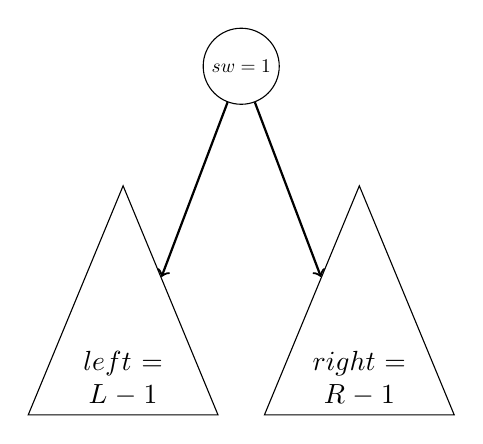
\begin{tikzpicture}
			\node[vertex](sw) at (0,1.5){$sw = 1$};
			\node[subtree](left) at (-1.5,0){$left = L - 1$};
			\node[subtree](right) at (1.5,0){$right = R - 1$};
	
			\draw[edge](sw) -- (right);
			\draw[edge](sw) -- (left);
		\end{tikzpicture}
		\caption{Their implementation takes the form of a binary tree. If the $sw$ bit is 1, then the value of $r$ is $L$ + $right$'s value.
		Otherwise the value of $r$ is $left$'s value.}
	\end{figure}
\end{frame}
\begin{frame}
	\frametitle{Aspnes, Attiya, Censor Implementation}
\begin{figure}[H]
    \begin{algorithmic}[1]
        \State $minRead()$
        \Indent
            \If{$switch = 0$} 
                \State \Return $left.minRead()$
            \Else
                \State \Return $right.minRead() + L$
            \EndIf
        \EndIndent   
    \alglinenoNew{alg2}
    \alglinenoPush{alg2}
    \end{algorithmic}
	\begin{algorithmic}[1]
		\alglinenoPop{alg2}
			\State $minWrite(v)$
			\Indent
				\If{$v < L$}
					\State $left.minWrite(v)$
					\State $switch \gets 0$ 
				\Else
					\If{$switch = 1$}
						\State $right.minWrite(v - L)$
					\EndIf
				\EndIf
			\EndIndent   
		\alglinenoPush{alg2}
		\end{algorithmic}
\end{figure}
\end{frame}

\begin{frame}
	\begin{figure}[H]
		\centering
		Suppose $L = 10$, $R = 10$, and we're implementing a 16-bounded min register.

		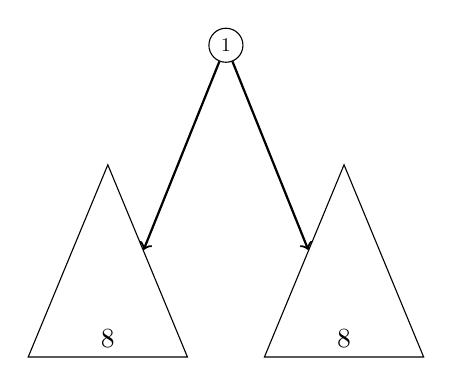
\begin{tikzpicture}
			\node[vertex](sw) at (0,1.5){$1$};
			\node[subtree](left) at (-1.5,0){$8$};
			\node[subtree](right) at (1.5,0){$8$};

			\draw[edge](sw) -- (right);
			\draw[edge](sw) -- (left);
		\end{tikzpicture}
		\caption{The min register initially looks like this.}
	\end{figure}
\end{frame}

\begin{frame}
	\begin{figure}[H]
		\centering
		After performing $r.minWrite(12)$, $r$ looks like this:
		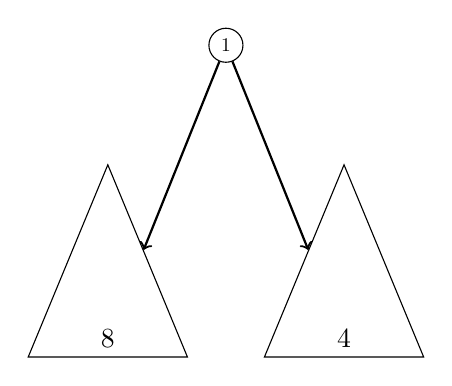
\begin{tikzpicture}
			\node[vertex](sw) at (0,1.5){$1$};
			\node[subtree](left) at (-1.5,0){$8$};
			\node[subtree](right) at (1.5,0){$4$};

			\draw[edge](sw) -- (right);
			\draw[edge](sw) -- (left);
		\end{tikzpicture}
	\end{figure}
\end{frame}


\begin{frame}
	\begin{figure}[H]
		\centering
		After performing $r.minWrite(3)$, $r$ looks like this:
		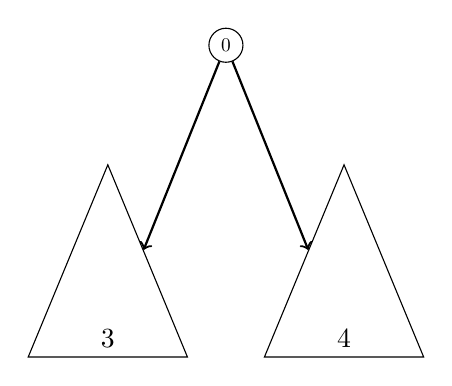
\begin{tikzpicture}
			\node[vertex](sw) at (0,1.5){$0$};
			\node[subtree](left) at (-1.5,0){$3$};
			\node[subtree](right) at (1.5,0){$4$};

			\draw[edge](sw) -- (right);
			\draw[edge](sw) -- (left);
		\end{tikzpicture}
		\caption{Essentially sw = 0 indicates that $r$'s value $< L$, and that $left$ holds the value of $r$.}
	\end{figure}
\end{frame}


\begin{frame}
	\begin{lemma}
	Suppose $left$ and $right$ are wait-free bounded min registers. Then so is $r$.
	\end{lemma}
	\begin{proof}
		The $r.minRead()$ and $r.minWrite()$ functions use only use a single step to either read or write to $sw$, in addition to using 
		the $minRead()$ and $minWrite()$ functions of $left$ and $right$. 
	\end{proof}
\end{frame}
\begin{comment}
\begin{frame}
	\begin{lemma}
		Suppose $left$ and $right$ are linearizable bounded min registers. Then so is $r$.
	\end{lemma}
	\begin{proof}
		Consider an execution in which every instance of $r.minRead()$ and $r.minWrite(v)$ instance
		is allowed to complete.\footnote{Given an incomplete execution $e$, since $r$ is wait-free, we can
		append an extension to allow incomplete instances to finish}

		\begin{itemize}
		\item Let $C_{right}$ be the set of $r.readMin()$ instances that read 1 from $sw$ and 
		$r.writeMin(v)$ ops that read 1 from $sw$ where $v > left.size$.
		\item Let $C_{left}$ be the set of $r.readMin()$ instances that read 0 from $sw$ and 
		$r.writeMin{v}$ ops with $v \le left.size$, and thus write $0$ to $sw$. 
		\item Let $C_{switch}$ be the set of $r.writeMin(v)$ that read 0 from $sw$ where $v > left.size$.
		\end{itemize}
	\end{proof}
\end{frame}

\begin{frame}
	\begin{proof}
		Observe that $C_{left}$ is exactly the set of instances that access $left$. 
		A $r.writeMin(v)$ instance in $C_{left}$ is linearized at the first instant $sw$ is 0 
		after is linearization point on its $left.writeMin(v)$, in the order these operations were linearized.
		\\~\
		In particular, every instance in $C_{switch}$ linearizes after the first such $r.writeMin(v)$
		instance in $C_{left}$ writes 0 to $sw$.  
		And thus these writes in $C_{switch}$ do nothing, since they linearize when $r$
		is already less than or equal to $left.size$.
		\\~\
		A $r.readMin()$ instance in $C_{left}$ is linearized at the same instant 
		that its $left.readMin()$ instance is linearized, before which it reads 0 from $sw$.
		Thus it linearizes after the first instance of $r.writeMin(v)$ in $C_{left}$ has linearized.
	\end{proof}
\end{frame}
\begin{frame}
	\begin{proof}
		Observe that $C_{right}$ is exactly the set of instances that access $right$.
		Every instance in $C_{right}$ is linearized in the same order as the order for their accesses to $right$,
		in either the configuration their access to right takes place or in the configuration before 0 is written to $sw$.
		Since every instance in $C_{right}$ reads 1 from $sw$, their linearization point lies within their operation
		and before any operation in $C_{left}$.
	\end{proof}
\end{frame}
 \begin{frame}
\frametitle{Linearizability proof}
	\begin{figure}
		\centering
		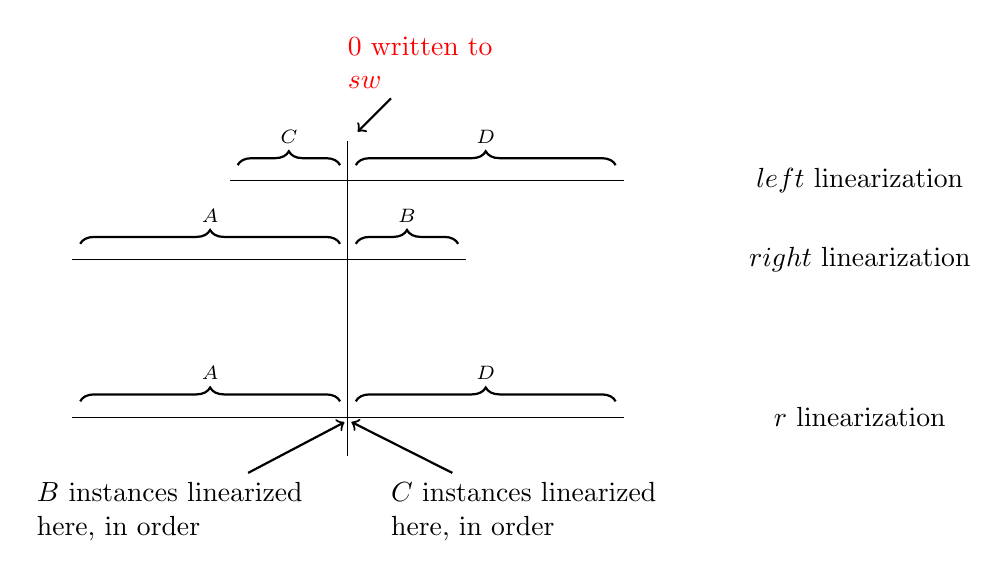
\begin{tikzpicture}[]
		%draw horizontal line
		\node(A) at (3.5,0.5){};
		\node[text width=2cm, color=red](B) at (4.5,1.5){0 written to $sw$};
		\draw[edge] (B) to (A);

		\draw (2,0) -- (3.5,0) -- (7,0); \node at (10,0){$left$ linearization};
		\draw (0,-1) -- (3.5,-1) -- (5.0,-1); \node at(10,-1){$right$ linearization};
		\draw (0,-3) -- (7,-3); \node at (10,-3){$r$ linearization};

		%draw vertical line to represent the write of 0 to sw
		\draw (3.5,0.5) -- (3.5,-3.5);
		\draw [thick ,decorate,decoration={brace,amplitude=5pt}] (2.1,0.2)  -- +(1.3,0) 
		node [black,midway,above=4pt, font=\scriptsize] {$C$};
		\draw [thick ,decorate,decoration={brace,amplitude=5pt}] (3.6,0.2)  -- +(3.3,0) 
		node [black,midway,above=4pt, font=\scriptsize] {$D$};
		\draw [thick ,decorate,decoration={brace,amplitude=5pt}] (0.1,-0.8)  -- +(3.3,0) 
		node [black,midway,above=4pt, font=\scriptsize] {$A$};
		\draw [thick ,decorate,decoration={brace,amplitude=5pt}] (3.6,-0.8)  -- +(1.3,0) 
		node [black,midway,above=4pt, font=\scriptsize] {$B$};
	   
		\draw [thick ,decorate,decoration={brace,amplitude=5pt}] (3.6,-2.8)  -- +(3.3,0) 
		node [black,midway,above=4pt, font=\scriptsize] {$D$};
		\draw [thick ,decorate,decoration={brace,amplitude=5pt}] (0.1,-2.8)  -- +(3.3,0) 
		node [black,midway,above=4pt, font=\scriptsize] {$A$};

		\node(C) at (3.58,-3.0){};
		\node[text width=3.5cm](D) at (1.3,-4.2){$B$ instances linearized here, in order};
		\draw[edge] (D) -- (C);
		\node(E) at (3.42,-3.0){};
		\node[text width=3.5cm](F) at (5.8,-4.2){$C$ instances linearized here, in order};
		\draw[edge] (F) -- (E);
		%draw vertical lines
		%\foreach \x in {0,2,5,7}{\draw (\x,3pt) -- (\x,-3pt);}
		%Draw nodes
		%\draw (0,0) node[above=3pt, text width = 3cm] { $w_{i+1}$ performs $R.update()$ } node[below=3pt] {(1)};
		%\draw (2,0) node[above=3pt, text width = 1.5cm] {$w_{i+x+1}$ finishes} node[below=3pt] {(2)};
		%\draw (5,0) node[above=3pt, text width = 3cm] { $w_i$ performs $R.update()$  } node[below=3pt] {(3)};
		%\draw (7,0) node[above=3pt, xshift=1cm,  text width = 3cm, color = red] {$w_{i+1}$ performs $R.update()$} node[below=3pt, color = red] {(1)};
		\end{tikzpicture}
		%\caption{}
	\end{figure}
\end{frame}
\end{comment}
\begin{frame}
	\frametitle{How can we implement this practically?}
	How can we implement this on a real machine?
\end{frame}
\begin{frame}
\frametitle{Practical Implementations of a $b$-bounded min register}
Idea 1: A $b$-bounded min register object stores the bit $sw$, 
and $left$, $right$ which are pointers to $\ceil{\frac{b}{2}}$ and $\floor{\frac{b}{2}}$-bounded min register objects respectively.
\\
Pros:
\begin{itemize}
	\item Very simple to implement.
	\item Might reduce memory contention to store bits in different objects at different places in memory
\end{itemize}
Cons
\begin{itemize}
	\item A lot of wasted space. On real machines, objects use at least 24 bytes per node used, so total space used is $24(b-1)$ bytes.
	\item Slow to traverse to different bounded min register objects from $left/right$.
\end{itemize}
\end{frame}
\begin{frame}
\frametitle{Practical Implementations of a $b$-bounded min register}
Idea 2: We can use a byte array-based tree, where each byte stores a switch register, and is the root of a subtree.
\end{frame}
\begin{frame}[fragile]
\frametitle{Array-based leveled binary tree}
\begin{definition}
	A binary tree is leveled if every row, except possibly the last is filled.
\end{definition}
We can use a $b$-byte array of atomic registers as a $b$ node leveled binary tree. 
In a leveled binary tree, the left child of a node at index $i$, if one exists, is at index $2i + 1$.
The right child, if it exists, is at index $2i + 2$.
\begin{figure}
	\begin{subfigure}[b]{0.47\textwidth}
	\centering
	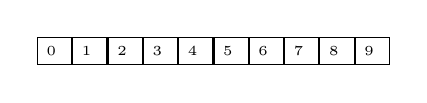
\begin{tikzpicture}
		\matrix [nodes={rectangle, draw=black, text width=2mm,anchor=west, font=\tiny }]
		{
			\node{0}; & \node{1}; & \node{2}; & \node{3}; & \node{4}; & \node{5}; & \node{6}; & \node{7}; & \node{8}; & \node{9}; \\
		};
	\end{tikzpicture}
	\hspace{10cm}
	\end{subfigure}
\hfill
	\begin{subfigure}[b]{0.47\textwidth}
	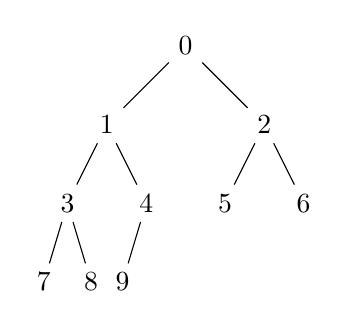
\begin{tikzpicture}
		\node(A) at (0,0){0};

		\node(B) at (-1,-1){1};
		\node(C) at (1,-1){2};

		\node(D) at (-1.5,-2){3};
		\node(E) at (-0.5,-2){4};
		\node(F) at (0.5,-2){5};
		\node(G) at (1.5,-2){6};

		\node(H) at (-1.8,-3){7};
		\node(I) at (-1.2,-3){8};
		\node(J) at (-0.8,-3){9};

		\draw (A) -- (B) -- (D) -- (H);
		\draw (A) -- (C) -- (G);
		\draw (D) -- (I);
		\draw (C) -- (F);
		\draw (B) -- (E) -- (J);
	\end{tikzpicture}
	\end{subfigure}
\end{figure}
\end{frame}
\begin{comment}
\begin{frame}
%size formula from integer sequences website....
The number of nodes in the left subtree in a leveled binary tree of size $n$:
\begin{align*}
	a(n) = He(n) \cdot (n + 2^{\floor{\log_2(n)}-1} - 1) + (-1)^{He(n)}\cdot(2^{\floor{\log_2(n)}} - 1)
\end{align*}
where 
\begin{align*}
	He(n) = H(-n + 3\cdot2^{\floor{\log_2(n)}-1} - 1) 
\end{align*}
and 
\begin{align*}
	H(x) = [x \ge 0]
\end{align*}
Proof by Bozinovski available here.
https://oeis.org/A279521
\end{frame}
\end{comment}
\begin{frame}
Pros:
\begin{itemize}
	\item More space efficient
\end{itemize}
Cons:
\begin{itemize}
	\item Now need $b-1$ bytes for a $b$-bounded register, which is still not great
\end{itemize}
\end{frame}
\begin{frame}[fragile]
\frametitle{But wait, there's more!}
We are only using 1 bit for every byte in the array...
What if instead we could use \emph{every bit} in the array rather than one per byte?
8 times the capacity!
\begin{itemize}
\item Before:
\\
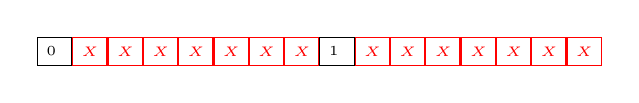
\begin{tikzpicture}
	\matrix [nodes={rectangle, draw=black, text width=2mm,anchor=west, font=\tiny }]
	{
		\node{0}; & \node[color=red]{$X$}; & \node[color=red]{$X$}; & \node[color=red]{$X$}; & \node[color=red]{$X$}; & \node[color=red]{$X$}; & \node[color=red]{$X$}; & \node[color=red]{$X$}; &
		\node{1}; & \node[color=red]{$X$}; & \node[color=red]{$X$}; & \node[color=red]{$X$}; & \node[color=red]{$X$}; & \node[color=red]{$X$}; & \node[color=red]{$X$}; & \node[color=red]{$X$}; \\
	};
	
\end{tikzpicture}

\item After:
\\
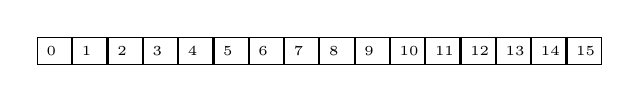
\begin{tikzpicture}
	\matrix [nodes={rectangle, draw=black, text width=2mm,anchor=west, font=\tiny }]
	{
		\node{0}; & \node{1}; & \node{2}; & \node{3}; & \node{4}; & \node{5}; & \node{6}; & \node{7}; &
		\node{8}; & \node{9}; & \node{10}; & \node{11}; & \node{12}; & \node{13}; & \node{14}; & \node{15}; \\
	};
\end{tikzpicture}
\end{itemize}
%bit array diagram
%TODO bit array diagram....
\end{frame}
\begin{frame}[fragile]
\frametitle{Reads and Writes to individual bits}
Reading a particular bit atomically is trivial. Can a byte and then use bitshifting.

But what about writing 0 to particular bit? We can use $fetch\&and$!

To write 0 to bit $i$ of a particular byte $a$ atomically, we can use $a.FAA(11111111_2 - (1 << (7 - i)))$ 
\end{frame}
\begin{frame}
	\frametitle{Optimizing number of steps}
	Notice that any reads occur before any writes in both minRead and minWrite operations.
	\begin{itemize}
		\item minReads will read switches before going down the tree
		\item minWrites will read switches before going down the tree and then write to switches on the way back up
	\end{itemize}
	We could read and write multiple switches at a time if they're in the same word in memory.
	So we could implement word size min registers in this way. But is there a better way?
\end{frame}

\begin{frame}
	\frametitle{Word sized min registers}
	When I mentioned that most computers have FAA, Faith came up with a better idea:

	Let $w$ be a word of $W$ bits such that the system supports FAA on $w$.
	\begin{itemize}
		\item We can implement a $(W+1)$-bounded min register from $w$.
		\item Initially, $w$ is all 1s.
		\item The value of $w$ at any time is the position of the rightmost off bit, or $W$ if all bits are on.
		\item A minRead will read $w$ and return the position of the rightmost off bit.
		\item A minWrite($v$) will use FAA to turn off the $v$-th bit, leaving the other bits unchanged.
	\end{itemize}
	This is a better implementation; minWrites now don't need to read, and we don't need to do any recursion or iteration to read/write 
	different bits.
\end{frame}

\begin{frame}
	\frametitle{Larger min registers that are slightly more efficient}
	What about for larger min registers? Notice that in the earlier implementation, $sw$ acts as a 2-bounded min register.
	It initially holds the value 1, and processes only read it or write 0 to it.
	\begin{itemize}
		\item What if we instead used our new word-size min register as the switch?
		\item Then we could use it to `pick' between $(W+1)$ subtrees which are each min registers, rather than 2.
		\item Reduces the step complexity of a $k$-bounded register from $\log_2(k)$ to $\log_{W+1}(k)$.
	\end{itemize}
\end{frame}
\begin{frame}
	\frametitle{Larger min registers that are slightly more efficient}
	Given we have words of size $W$ and $S$-bounded min registers,
	\begin{itemize}
		\item We use a $(W+1)$-bounded min register $sw$, as the switch,
		\item and $(W+1)$ $S$-bounded min registers, $tree_0 \dots tree_W$,
		\item to obtain a $(W+1)S$-bounded min register $r$.
	\end{itemize}
\end{frame}

\begin{frame}
	\begin{figure}[H]
		\begin{algorithmic}[1]
			\State $minRead()$
			\Indent
				\State $i \gets sw.minRead()$ 
				\State \Return $tree_i.minRead() + is$
			\EndIndent 
		\alglinenoNew{alg3}
		\alglinenoPush{alg3}
		\end{algorithmic}
		\begin{algorithmic}[1]
			\alglinenoPop{alg3}
				\State $minWrite(v)$
				\Indent
					\State $d \gets \floor{\frac{v}{S}}$
					\State $i \gets sw.minRead()$ 
					\If{$i \ge d$}
						\State $tree_d.minWrite(v - d \cdot S)$
						\If{$i > d$}
							$sw.minWrite(d)$
						\EndIf
					\EndIf
				\EndIndent   
			\alglinenoPush{alg3}
			\end{algorithmic}
	\end{figure}
\end{frame}


\begin{frame}
	\begin{figure}[H]
		\centering
		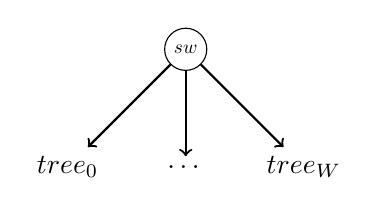
\begin{tikzpicture}
			\node[vertex](sw) at (0,1.5){$sw$};
			\node(zero) at (-1.5,0){$tree_0$};
			\node(w) at (1.5,0){$tree_W$};
			\node(dots) at (0, 0){$\dots$};

			\draw[edge](sw) -- (zero);
			\draw[edge](sw) -- (dots);
			\draw[edge](sw) -- (w);
		\end{tikzpicture}
	\end{figure}
\end{frame}

\begin{frame}
	\frametitle{Open question}
		In both implementations, a wait-free $b$-bounded min register requires $b-1$ bits and has $O(\log b)$ step complexity.
		Is there an implementation that uses fewer bits that has $O(\log b)$ or better step complexity?
\end{frame}
\begin{frame}
	\frametitle{Open questions}
	While technically wait-free, brute force implementations from CAS are slow. Given a word $w$ of $W$ bits, 
	we could implement a $2^W$ bounded min register as follows:
	\begin{itemize}
		\item A minRead would return the current value of $w$.
		\item A minWrite($v$) would read the current value $c$ of $w$, and if $c$ is greater than $v$, 
		perform $w.CAS(c,v)$, repeatedly trying until the value of $r$ less than $v$.
	\end{itemize}
	The step complexity of minWrites in this implementation would be $O(b-v)$, since a $minWrite$ might have to perform a $b-v-1$ CAS operations on $w$
	before $w$ holds a value that is less than or equal to $v$. Other processes could perform CAS($2^W - 1$,$2^W - 2$), CAS($2^W - 2$,$2^W - 3$), etc....
\end{frame}

\end{document}
